\usepackage[utf8]{inputenc}
\usepackage[french]{babel}
\usepackage{csquotes}
\usepackage[T1]{fontenc}
\usepackage{geometry}
\geometry{a4paper,width=160mm,top=20mm,bottom=20mm,bindingoffset=6mm}
\usepackage{graphicx}
\usepackage[scleft,ruled,french]{algorithm2e}
% \usepackage{algorithm}
% \usepackage{algcompatible}
\usepackage{amsmath}
\usepackage{amssymb}
\usepackage{amsthm}
\usepackage{fancyhdr}
\usepackage{hyperref}
\usepackage{float}
\usepackage{lscape}
\usepackage{array}
\usepackage[normalem]{ulem} % https://github.com/plk/biblatex/issues/193
% \usepackage{import}
\usepackage{afterpage}
\usepackage{xcolor}
\usepackage{tikz}
\graphicspath{{images/}}
% \usepackage{listings}
\usepackage{longtable}
\usepackage{rotating}
\usepackage[nottoc]{tocbibind}
\usepackage[backend=biber,sorting=none]{biblatex}
\usepackage{pdfpages}
\usepackage{subfiles}
\usepackage{caption}
\usepackage{subcaption}
\usepackage{tabularx}



\renewcommand{\thetable}{\Roman{table}}
\renewcommand{\headrule}{
    \vspace{-15pt}
    \hrulefill\ 
    \raisebox{-0pt}{
        \scalebox{0.3}{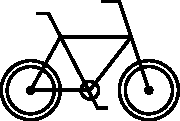
\includegraphics{PDFs/bike.pdf}}
    }
    \hrulefill
}

\setlength{\headheight}{24pt}
\pagestyle{fancy}
\fancyhf{}
% \fancyhead[LE]{\nouppercase{\rightmark\hfill\leftmark}}
\fancyhead[C]{INSA Rouen \hfill LIFAT}
\fancyfoot[C]{\hfill \thepage \hfill}

%lien
\hypersetup{
    colorlinks=true,
    linkcolor=black,
    filecolor=magenta,     
    urlcolor=blue,
    citecolor=blue,
}

\DeclareMathOperator{\Maximize}{Maximize}
\DeclareMathOperator{\Minimize}{Minimize}
\newcommand{\fFrac}[2]{%
	\mathchoice
	{\raisebox{0.4ex}{\ensuremath{#1}} \kern-0.1em/\kern-0.1em\raisebox{-0.4ex}{\ensuremath{#2}}}% displaystyle
	{\raisebox{0.4ex}{\small\ensuremath{#1}} \kern-0.1em/\kern-0.1em\raisebox{-0.4ex}{\small\ensuremath{#2}}}% textstyle
	{\raisebox{0.4ex}{\footnotesize\ensuremath{#1}} \kern-0.1em/\kern-0.1em\raisebox{-0.4ex}{\footnotesize\ensuremath{#2}}}% scriptstyle
	{\raisebox{0.4ex}{\scriptsize\ensuremath{#1}} \kern-0.1em/\kern-0.1em\raisebox{-0.4ex}{\scriptsize\ensuremath{#2}}}% scriptscriptstyle
    }

%aconfig algorithme
\SetKwInput{Donnees}{Données}
\SetKwInput{Res}{Résultat}
\SetKwInput{Renvoyer}{Renvoyer}
\SetKwComment{Comment}{\# }{}
\SetKwFor{Pour}{pour}{faire}{fin pour}
\SetKwFor{PourCh}{pour chaque}{faire}{fin pour chaque}
\SetKwIF{Si}{SinonSi}{Sinon}{Si}{alors}{Sinon si}{Sinon}{fin si}
\SetKwFor{TantQue}{tant que}{faire}{fin tant que}